% Name: Max pooling
% Description: A 2 by 2 max pool with stride 2: each colored block of the 4 by 4 input keeps only its largest value.
% Tags: max pooling, downsampling, CNN, feature map

\usetikzlibrary{arrows.meta}

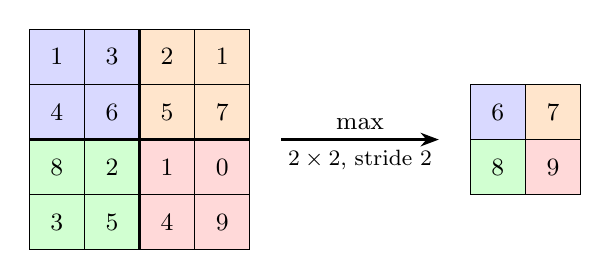
\begin{tikzpicture}[cell/.style={draw, minimum size=7mm, inner sep=0pt, font=\small}]
  \foreach \x/\y/\c in {0/0/blue!15, 1.4/0/orange!20, 0/-1.4/green!18, 1.4/-1.4/red!15}
    \fill[\c] (\x,\y) rectangle ++(1.4,-1.4);
  \foreach \row [count=\r from 0] in {{1,3,2,1}, {4,6,5,7}, {8,2,1,0}, {3,5,4,9}}
    \foreach \v [count=\c from 0] in \row
      \node[cell] at (0.7*\c+0.35, -0.7*\r-0.35) {\v};
  \draw[very thick] (1.4,0) -- (1.4,-2.8) (0,-1.4) -- (2.8,-1.4);
  \draw[-{Stealth}, thick] (3.2,-1.4) -- node[above, font=\small] {max} node[below, font=\footnotesize] {$2\times 2$, stride 2} (5.2,-1.4);
  \foreach \v/\x/\y/\c in {6/0/0/blue!15, 7/1/0/orange!20, 8/0/1/green!18, 9/1/1/red!15}
    \node[cell, fill=\c] at (5.95+0.7*\x, -1.05-0.7*\y) {\v};
\end{tikzpicture}
